\documentclass[output=paper]{langscibook}
\ChapterDOI{10.5281/zenodo.12090445}
\abstract{This paper presents some evidence that language change in heritage languages (and beyond) systematically responds to general factors of language design when it comes to fixed sequences of functional heads within given domains. Concretely, we investigate patterns of change across various heritage languages, both in the word-internal domain (person and number features) and at the sentence level (word order): we show that change in these different domains is consistently shaped by a bias towards monotonicity and uniformity in computation, such that points of non-uniformity in the relevant sequence can be predicted to be the gateway to change. Crucially, this change systematically brings about a reduction in complexity; as such, these factors are proposed as a new metric for linguistic complexity.}



\title{Non-monotonic functional sequences: A new metric for complexity in heritage languages}
\author{Roberta D'Alessandro\affiliation{Utrecht University} and Silvia Terenghi\affiliation{Utrecht University}}

\IfFileExists{../localcommands.tex}{
  \addbibresource{../localbibliography.bib}
  \usepackage{tabularx,multicol}
\usepackage{url}
\urlstyle{same}
\usepackage{multirow}

\usepackage{stmaryrd}
\usepackage{soul}
\usepackage{enumitem}

\usepackage{siunitx}
\sisetup{group-digits=none}

\usepackage{langsci-optional}
\usepackage{langsci-lgr}
\usepackage{langsci-textipa}
\usepackage{langsci-branding}

\usepackage{tikz-qtree}

\usepackage{pgfplots}
\usepackage{qtree}
\qtreecenterfalse
\usepackage{tree-dvips}
\usepackage{subcaption}

\let\clipbox\undefined
\usepackage{adjustbox}
\usepackage[linguistics, edges]{forest}
\usepackage{langsci-gb4e}

% ORCIDs in langsci-affiliations 
\usepackage{orcidlink}
\SetupAffiliations{orcid placement=before}
\definecolor{orcidlogocol}{cmyk}{0,0,0,1}
\RenewDocumentCommand{\LinkToORCIDinAffiliations}{ +m }
  {%
    \orcidlink{#1}\,%
  }

  \newcommand*{\orcid}[1]{}


\makeatletter
\let\thetitle\@title
\let\theauthor\@author
\makeatother

\newcommand{\togglepaper}[1][0]{
   \bibliography{../localbibliography}
   \papernote{\scriptsize\normalfont
     \theauthor.
     \titleTemp.
     To appear in:
     E. Di Tor \& Herr Rausgeberin (ed.).
     Booktitle in localcommands.tex.
     Berlin: Language Science Press. [preliminary page numbering]
   }
   \pagenumbering{roman}
   \setcounter{chapter}{#1}
   \addtocounter{chapter}{-1}
}

\newbool{bookcompile}
\booltrue{bookcompile}
\newcommand{\bookorchapter}[2]{\ifbool{bookcompile}{#1}{#2}}


\forestset{
  my nice empty nodes/.style={% modified from manual page 52
    for tree={
      calign=fixed edge angles,
      calign angle=50,
    },
    delay={
      where n children=0{
        if content={}{
          content=\strut,
          anchor=north,
        }{
          align=center
        },
      }{
        if content={}{
          shape=coordinate,
          for parent={
            for children={
              anchor=north
            }
          }
        }{}
      }
    },
  },
  my pretty nice empty nodes/.style={
    for tree={
      calign=fixed edge angles,
      calign angle=50,
      parent anchor=south,
      delay={
        where n children=0{
          if content={}{
            content=\strut,
            anchor=north,
          }{
            align=center
          },
        }{
          if content={}{
            inner sep=0pt,
            edge path={\noexpand\path [\forestoption{edge}] (!u.parent anchor) -- (.south)\forestoption{edge label};}
          }{}
        }
      }
    }
  }
}


\newcommand{\sem}[1]{\mbox{$[\![$#1$]\!]$}}
\newcommand{\type}[1]{\ensuremath{\left \langle #1 \right \rangle }}
\newcommand{\lam}{\ensuremath{\lambda}}
\renewcommand{\and}{$\wedge$ }
\newcommand{\bex}{\begin{exe}}
\newcommand{\eex}{\end{exe}}
\newcommand{\bit}{\begin{itemize}}
\newcommand{\eit}{\end{itemize}}
\newcommand{\ben}{\begin{enumerate}}
\newcommand{\een}{\end{enumerate}}

\newcommand{\gcs}[1]{\textcolor{blue}{[gcs: #1]}}
\newcommand{\ash}[1]{\textcolor{orange}{[ash: #1]}}
\newcommand{\ngn}[1]{\textcolor{purple}{[ngn: #1]}}

\newcommand{\firstrefdash}{}


\forestset{
fairly nice empty nodes/.style={
delay={where content={}
{shape=coordinate, for siblings={anchor=north}}{}},
for tree={s sep=4mm}
}
}



  %% hyphenation points for line breaks
%% Normally, automatic hyphenation in LaTeX is very good
%% If a word is mis-hyphenated, add it to this file
%%
%% add information to TeX file before \begin{document} with:
%% %% hyphenation points for line breaks
%% Normally, automatic hyphenation in LaTeX is very good
%% If a word is mis-hyphenated, add it to this file
%%
%% add information to TeX file before \begin{document} with:
%% %% hyphenation points for line breaks
%% Normally, automatic hyphenation in LaTeX is very good
%% If a word is mis-hyphenated, add it to this file
%%
%% add information to TeX file before \begin{document} with:
%% \include{localhyphenation}
\hyphenation{
    par-a-digm
    peri-phras-tic
    mor-pho-pho-nol-o-gy
}

\hyphenation{
    par-a-digm
    peri-phras-tic
    mor-pho-pho-nol-o-gy
}

\hyphenation{
    par-a-digm
    peri-phras-tic
    mor-pho-pho-nol-o-gy
}

  \togglepaper[1]%%chapternumber
}{}

\shorttitlerunninghead{Non-monotonic functional sequences}
\begin{document}
\SetupAffiliations{mark style=none}
\shorttitlerunninghead{Non-monotonic functional sequences}
\maketitle


\section{Introduction}

Complexity is a recurrent concept in the analysis of heritage grammars. Nonetheless, a rigorous, agreed upon definition of complexity is currently lacking. In this paper, we restrict the focus to a specific set of purely syntactic phenomena, the derivation of which can be taken to hinge on feature sequences. We show that, when fixed sequences of functional heads are concerned, complexity can be understood as a correlate of properties inherent to this sequence, and more specifically to their values. We identify two general factors of language design: (i) bias towards monotonicity and (ii) uniformity in computation; building on these, we show that it is possible to predict that points of inconsistency across the relevant feature values (from $+$ to $-$ and from $-$ to $+$) will be the gateway to change in heritage languages, as well as in other forms of change, most notably spontaneous, diachronic change.

We first provide an overview on complexity in general and in heritage languages (HLs henceforth) in particular (Section \ref{sec:compl}). We further argue that the concept of complexity needs to be related to the monotonicity profile of the relevant functional sequence. With this background in place, we explore the proposal by considering two domains, each related to one specific sequence of elements. Section \ref{sec:word} discusses phenomena at the word-internal level, where the hypothesis is illustrated by means of heritage grammars that display change in the person and number domains. In Section \ref{sec:sentence}, instead, the hypothesis is illustrated additionally by considering the phenomena at the sentence level, and more specifically word order facts as found across heritage languages. Section \ref{sec:concl} concludes.


\section{Complexity in heritage languages\label{sec:compl}}

Heritage languages are defined in different ways depending, among other factors, on various linguistic traditions. Minority languages that are in balanced or displacive contact with a majority language spoken in a given area, as well as dialects or variants of the same language, and languages spoken by immigrants' children, all fall into the category of HLs.\footnote{According to the typological tradition of contact studies, \textit{balanced contact} obtains ``in a situation of a long-standing linguistic area and stable multilingualism without any dominance relationships'' (\citealt[42]{Aikhenvald2006}); \textit{displacive contact} happens instead ``if one group aggressively imposes its language on another group, [resulting] in language displacement, loss of the language's own features, and, ultimately, language shift'' (\citealt[43]{Aikhenvald2006}).} In this paper, we will use the tag HL to refer mostly to those languages spoken by the children of immigrants, learned in a naturalistic environment, for instance at home or within a small community, but crucially different from the dominant/official language(s) spoken in the larger community that they are part. Quoting \citet[9]{Polinsky2018}, ``[a] heritage language speaker (for short, heritage speaker) is a simultaneous
or sequential (successive) bilingual whose weaker language corresponds to the minority language of their society and whose stronger language is the dominant language of that society''.

The study of HLs has developed in different directions in the last few years: on the one hand, focus has been put on the divergence of HL grammars from so-called baseline grammars (see at least discussion in \citealt[1.3.3]{Polinsky2018} for the concept of divergent attainment; \citealt{PiresRothman2009} for that of missing-input competence divergence; and \citealt{Montrul2008} for that of incomplete acquisition); on the other hand, focus has been put on the speaker's mastery of the language processes (starting from the Shallow Structure Hypothesis by \citealt{ClahsenFelser2006}, and especially studies involving interfaces, e.g. \citealt{Sorace2011}). Yet another path is taken by studies like \citet{Bayrametal2019}, which take into account the role of inter-generational attrition in HL acquisition, and put emphasis on the fact that ``divergent'' attainment could be due to exposure to qualitatively different input with respect to monolingual learners.

This paper takes a slightly different viewpoint, by focusing exclusively on the grammatical system of HLs, putting aside all considerations on performance, onset, fluency, number of languages spoken and their order of acquisition. Our aim is to identify general principles that govern HLs and constrain the ways in which they deviate from the relevant baseline for comparison (for which, see Section \ref{sec:basel} below). In other words, our aim is to discuss some principles of language change, where language is intended as grammar.

\subsection{The problem of the baseline\label{sec:basel}}

Whether the focus is on the grammar or on the speaker, HLs have typically been tackled in a comparative fashion: how has a given HL changed (i.e., how has it become simpler or more complex) with respect to its baseline? And what is this change due to? 

When trying to understand the mechanisms behind language change, the first problem is to define the system against which grammatical change can be assessed. This is a well-known issue, usually referred to as the ``baseline problem'' (for an overview of the baseline problem, see \cites[1.1.2]{Polinsky2018}[Ch. 6]{AalberseMuysken2019}{Bayrametal2019}{DAlessandroEtAl2021}). Identifying the baseline is not an easy task, especially when dealing with minority and/or non-standardized languages. For example, is the baseline for Heritage Italian spoken in the US the Italian spoken in Italy today? Or is it rather the language to which the heritage speakers were exposed during acquisition? The ``deviating value'' which appears to be the result of language change might have already been present in the baseline, for instance because the original variety was not standardized and presented wide microvariation. If this original microvariation is not documented to start with, identifying change in non-standardized varieties becomes nearly impossible. A further issue regards the fact that HLs are often compared to their contemporary counterparts in the language homeland, and not, for instance, to the varieties that were spoken in the country of origin at the moment in which the emigrants left them.

The problems just mentioned make the issue of identifying change more difficult to tackle in the absence of a clear understanding of the underlying mechanisms of change. While HL studies are a subset of bilingualism studies, we need to understand the underlying mechanisms guiding change and constraining it. In the absence of a clear view on such mechanisms, we are left with no guidance as to what is possible (and can possibly have been the result of language change) and what is not. A similar \textit{desideratum} has been recently expressed by \citet{Polinsky22}: describing some phenomena that underwent change, ``itemizing tokens of change'', so to say, is not going to bring us too far, if we do not identify some general laws governing said change. These laws can help us solve the issue regarding the possible input for a given phenomenon, in the absence of empirical evidence indicating where the change started from.

In this paper, we will present one such underlying law, identified not only on the basis of HLs, but also on the basis of diachronic evidence. This law, which we call the \textit{monotonicity bias}, seems to inform language change in contact as well as in diachrony. We will present some case studies, at both the word and sentence levels, focusing on HLs. More concretely, we will argue that HLs tend toward simplification, but only in those areas of language directly related to grammatical features. Before moving on to the discussion of the case studies, we briefly touch upon the definition of simplification and complexification in language change. 

One of the tendencies that have been pointed out for HL grammars is that they are significantly less complex than their corresponding baseline (see \citealt{PolinskyScontras2020} for discussion).\footnote{From now on, we will simply refer to the baseline as the system against which we observe change, bearing in mind what was discussed in the beginning of the section.} This has been attributed to different factors, including: HL speakers tend to avoid ambiguity/indeterminacy (\citealt[5.2]{Polinsky2018}; the ``ambiguity problem'' in \citealt{PolinskyScontras2020}), for instance by avoiding polyfunctional words; they avoid silence (the so-called ``silence problem'': \citealt{LalekoPolinsky2017}; \citealt[6.5]{Polinsky2018}). However, from a strictly grammatical viewpoint, it is not obvious what this ``simplification'' amounts to, or whether we can talk of simplification at all, in the first place. Here, we will not use the term ``simplification'' with respect to performance-based phenomena: as stated above, we will focus exclusively on structure. To do this, we need to briefly discuss the concepts of complexity and markedness; subsequently, we will outline a system predicting functional feature-related change and present evidence for it.

\subsection{Complexity and markedness\label{sec:m}}

Complexity is an elusive concept. If the aim is to determine whether complexity has increased or reduced in a system, one needs to have a way to quantify complexity in order to measure it. There have been attempts to measure complexity, both for HLs (for an overview, see \citetv{chapters/varatharaj}) and for languages in general. 

One thing to bear in mind is that, although complexity and markedness are obviously very different concepts, complexity has often been reduced to markedness, with the underlying assumption that more marked elements are more complex. Observe that, while markedness traditionally refers to one item or one paradigm, and is determined as a difference with respect to the rest of the system, complexity usually refers to the system as a whole, and is determined by means of comparisons between systems. Markedness of several forms in a system can result in the system being more complex, for instance. This idea has been informed by the same observation regarding the decrease of complexity in diachronic linguistics: languages tend to eliminate complexity through time, and marked elements are also eliminated by the system through time. Something similar has been claimed, on different channels, in contact studies, for instance those on creolization (see for instance \citealt{McWhorter2001}, among many others). 

The correspondence between complexity and markedness is somehow intuitively right, but it suffers from some flaws that have been highlighted by many, among which is \citet{Haspelmath2006}. In a qualitative fashion, \citeauthor{Haspelmath2006} underlines that markedness has different meanings when related to different aspects, and that simplification in one area can mean complexification in another (in this respect, his conclusions are not different from those in \citeauthor{chapters/varatharaj}, this volume). %\citealt{Scontras2022}). 
Consider for instance a clitic-left dislocation construction in Standard Italian, like the one in (\ref{clld}):
\begin{exe} 
\ex \begin{xlist}
\ex \label{clld}\gll 
La torta l'hai          mangiat-a\\
the cake it=have.\textsc{2sg}   eaten-\textsc{f.sg} \\
\glt `The cake, you ate it.'
\ex \gll 
Hai mangiat-o la torta \\
have.\textsc{2sg} eaten-\textsc{m.sg} the cake \\
\glt `You ate the cake.'
\end{xlist}
\end{exe}
(\ref{clld}) is quite transparent from a discourse viewpoint, with the object appearing first in the sentence, which makes it immediately clear that one is talking about a cake, the topic. However, if we look at syntactic complexity in terms of number of syntactic operations, the situation is reversed: the object is left-dislocated (which means that a movement operation is required); this object dislocation also triggers agreement, which is absent when the object is \textit{in situ}. Simplification in interpretation and understanding of discourse corresponds to complexification in syntactic operations, very often also reflected in slowness of processing because of the establishment of a dependency between the object and the clitic (see for instance \citealt{ValleHootCabrelli}). This means that we need to identify not just a measure of complexity, but also the domain in which complexity is assessed. 

Regarding the idea of exploiting markedness to identify complexity, it needs to be recalled that the concept of \textit{markedness} was first introduced by Trubetzkoy and Jakobson in the 1930s (\citealt{Trubetzkoy31, Trubetzkoy39, Jakobson32, Jakobson39}), and was mainly used to refer to the characteristics of a grammatical item. As an example, consider the voiced/voiceless alternations in consonants: voiced consonants have, according to Jakobson, an additional “specification” compared to voiceless consonants. From this perspective, “while the optimal consonant is voiceless and the optimal vowel is voiced, the voicing of consonants and, in very rare instances, the unvoicing of vowels, may be utilized as one of the various phonetic attenuations of the maximum contrast CV” \citep[56--57]{JakobsonHalle56}. According to this line of thought, that the voiceless consonants are unmarked is also shown by the existence of final devoicing rules, ``erasing'' the voice\slash marked feature, in languages like Russian. The markedness on one item has been exploited very often to investigate ``morphological complexity''. 

An example of morphological markedness which is difficult to master for HL speakers can be the Italian finite verb inflectional morphemes, which encode information about the person and number of the subject, as well as the tense, aspect and mood of the verb. These morphemes are semantically marked, since they contain many meanings, and also morphologically marked, because these meanings that are mapped to one exponent simultaneously are not immediately identifiable as the morphology is often ``irregular''. HLs tend to move in the direction of simplification of semantic complexity in the inflectional system. In a recent study, \citet{AndrianiDAlessandro22} show that the inflectional systems of Italo-Romance HLs in the Americas are heavily reduced: speakers pick one of the two strategies: they either replace the inflected form with a default one (like the 3rd person singular form of the present tense) or they delete the auxiliary altogether. A similar process is found in creole languages like Papiamento, where the auxiliary only encodes tense (\textit{ta} for the present tense vs. \textit{a} for the past tense) but no \textit{phi}-agreement features.

Morphological markedness can also be tackled from a paradigmatic viewpoint, for instance by isolating the verbal paradigm in a language L and checking how many overt inflectional forms it includes. The more inflectional forms a paradigm contains, the more marked it will be. The more inflecting categories a language has, the more complex (at least, morphologically) the language is. This position is adopted by \citet{nichols1992}, who defines complexity in terms of inflecting categories in a language. 
Observe that if the mapping between the exponent and its meaning is a bijective function, this does not indicate necessarily more complexity: the system is richer, but transparent, therefore not necessarily harder to master. 


In the remainder of the chapter we will build on intuitions related to morphological complexity, but we will not be adopting this approach to quantify complexity. Rather, we propose a definition of complexity based on morphological structure, taking features and the sequence of functional heads which constitute words as its primitives, in conformity with our task, i.e. to identify an underlying principle governing complexity and simplification in language change. More concretely, we put forth one such underlying principle, namely what we call the \textit{monotonicity bias} (\citealt{Terenghi2021LAGB, Terenghi2022Sinf15, Terenghi2023}: 173 ff.). We will base our analysis on the kind of markedness which \citet{Haspelmath2006} dubs as ``markedness as default from parametric settings'', stemming from \citet[Ch. 9]{ChomskyHalle1968} and \citet{Kean1975}. The basic idea is that markedness is given by ``the odd one out'' with respect to a system.
These diagnostics could be easily put to use to identify the mechanisms of language change, in at least two ways. The first way would be to actually count the number of irregular words in a language, and check whether they are systematically replaced by regular forms. This seems to be the case in HL, according to what is reported by \citet{AalberseMuysken2019}. The second way would be to extend these considerations to all grammar modules, and for instance establish a correspondence between portmanteau morphs at the morphological level and complex functional heads, encoding more than one piece of semantics, at the syntactic level. Consider again the tense head in Romance: this head is considered to encode at the same time tense, aspect, mood, and \textit{phi}-features. It is a ``portmanteau'' functional head, which parallels its morphological counterpart. Does some of the information on this head tend to disappear, or does it become more inconsistently marked, or does it settle on a reduced form? Does subject agreement disappear, or does it reduce? Does mood disappear? All these questions have been posed in HL studies, and have been given positive answers: see, for instance, \citet{vanOschSleeman2018Spanish} on the disappearance of subjunctive in heritage Spanish spoken in the Netherlands. While we do seem to have collected quite a large amount of evidence in favour of simplification of functional heads, the principle underlying this simplification is still obscure. 

To understand what this means, we borrow an example from \citet{RobertsHolmberg2010} on word order in Japanese, a head-final language. Under the assumption that head-finality is reached through movement to the specifier of dedicated functional heads, and that movement is a costly operation (contra \citealt{Chomsky2013}, as well as from a processing\slash interpretational viewpoint), a verb-final language should be more marked than a verb-initial language. The standard assumption regarding movement in minimalist syntax is that it is triggered by an EPP-feature on functional heads, which attracts the moving XP to the specifier of the head featuring the [EPP]. Considering this, head-final languages should be very marked, as they would need an ``extra'' EPP-feature on every head. Languages like German or Latin, with mixed word order, might be considered as partially marked, given that not all heads would require the EPP-feature, and harmonically head-initial languages like Italian or English would be unmarked. 

Building on \citet{ChomskyHalle1968}, however, \citet{RobertsHolmberg2010} reconsider markedness not as arising from the presence of an additional feature on one functional head but, more holistically, as resulting from a deviation from the paradigm, which in the case of syntax is identified in the set of all functional heads of a language. Through this lens, harmonic head-final languages like Japanese are not marked systems at all, as every functional head carries an EPP-feature. Likewise, consistently head-initial languages are not marked, as no functional head carries an EPP-feature. The only marked systems are those that give origin to disharmonic word orders, like that of German for instance, where head-finality and head-initiality are both present in the system because the EPP-feature is present only on some functional heads, and its distribution depends on whether the clause is a root or embedded one. 

\citet{RobertsHolmberg2010} conclude that the preference for harmonic ordering seems to derive from an overriding tendency for independent parameters to conspire to produce a certain type of grammar. This intuition had already been expressed, in functional terms, by \citet{Hawkins1983} under the notion of cross-categorial harmony, whereby languages are preferred if their constituents display a harmonic ordering. \citet[39--40]{RobertsHolmberg2010} rephrase this proposal as in (\ref{ex:EPP1}) and, more formally, in (\ref{ex:EPP2}):
\begin{exe}
\ex \begin{xlist}
\ex There is a preference for the EPP-feature of a functional head F to generalise to other functional heads G, H ...\label{ex:EPP1}
\ex \label{ex:EPP2} For a class of heads H, \textit{u}EPP for H$_{\textrm{F}:-}$ $\neq$ \textit{v} $\rightarrow$ \adjustbox{valign=t}{\begin{tabular}{lll}
\multirow{2}{*}{$\biggl\{$} & \hspace*{-.3cm}{[}$+$EPP]/\textit{v}$_{+\textrm{EPP}}$; & \hspace*{-.3cm}\parbox[t]{2mm}{\multirow{2}{*}{\rotatebox[origin=c]{180}{$\biggl\{$}}}\\
& \hspace*{-.3cm}{[}$-$EPP] elsewhere &\\
\end{tabular}}
\end{xlist} 
\end{exe}
							    
\noindent In summary, for some languages, the unmarked value for the functional heads is [$+$EPP]. These are OV-languages, where the object is attracted across the verb to the specifier of a higher functional head. For some other languages, the unmarked value for the probe heads is [$-$EPP]. These are the VO-languages. Mixed systems, disharmonic word orders, where the EPP-feature is present on only some heads, are more marked (see also \citealt{BiberauerSheehan2013}).

\citet[41]{RobertsHolmberg2010} propose that this tendency toward uniformity is also the driving principle behind the acquisition of word order. Learners exploit pieces of input, focusing their attention in particular on the \textit{v} head, which is the core head in a clause as it encodes transitivity. Once the [EPP] value on \textit{v} is identified, it gets transferred to all the other functional heads in grammar, according to a mechanism called the Generalization of the input explicated in (\ref{inputgen}):
\begin{exe}
\ex Generalization of the input (\citealt[41]{RobertsHolmberg2010})\\
If acquirers assign a marked value to H, they will assign the same value to all comparable heads. \label{inputgen}
\end{exe}
Our analysis of complexity will build heavily on Robers \& Holmberg's (\citeyear{RobertsHolmberg2010}) intuitions: we will show that language change in contact, in particular in HLs, tends toward unmarked systems, i.e. systems that only include functional heads with the same value. We will call them \textit{monotonic}. 
Before delving into monotonicity, a last methodological note is required. An observation borrowed from classical phonological studies, like \citet{ChomskyHalle1968} or \citet{Kean1975}, is that markedness arises ``one step at a time''. In phonological terms, for instance, starting from the fact that all languages have an /a/, the next step will be to add height, and therefore there will be systems with /a/, /i/, and /u/; then, anteriority will be added, and so on, but crucially markedness will not jump ahead and skip one of these steps. We observe the same mechanism in the uniform restructuring of functional sequences: it will be shown that this kind of simplification takes place one step at a time, along the functional sequence. 

\subsection{(Non-)monotonic functional sequences}

We first start by assuming that whenever the derivation of a given phenomenon can be shown to exclusively hinge on an underlying sequence of features, properties inherent to that sequence will determine the complexity level for the given phenomenon: more specifically, sequences of features that only include functional heads that share one and the same value (harmonic, in Roberts \& Holmberg's terms) are regarded as less complex than sequences of features that include functional heads with different values (disharmonic). Distinct from \citeauthor{RobertsHolmberg2010}, however, we extend this proposal to the word-internal level, too. This allows us to find a previously unnoticed parallelism across the nominal and the clausal domain, as in both cases the gateway for change within the system can be shown to be exactly the point of the sequence where the relevant features switch values. We refer to sequences that involve such switches as non-monotonic sequences and propose that they are more complex due to a general bias towards monotonic computation.

\begin{sloppypar}
Monotonicity is a property whereby (mathematical) functions do not vary in tone for a given value's interval. Monotonic functions are either entirely non-decreasing (monotonically increasing functions) or entirely non-increasing (monotonically decreasing functions); functions that instead are partly increasing and partly decreasing can be defined as non-monotonic. The general rationale behind the notion is that, given a partial order within a domain, monotonicity consistently preserves it or reverses it. In this sense, monotonicity has been shown to be also relevant beyond the mathematical level, for other cognitive modules. Interestingly, monotonicity shapes language, too, and it most famously does so in the domain of quantifiers. This line of research goes back at least to \citet{BarwiseCooper1981}, where the relevant partial ordering is the one that exists between two sets that stand in a subset--superset relation.
\end{sloppypar}

In this paper we extend this notion to the \textit{phi}-features domain in syntax (based on \citealt{Terenghi2021LAGB, Terenghi2022Sinf15, Terenghi2023}). We assume an action-on-lattice semantics for person and number features (\citealt{Harbour2008, Harbour2014, Harbour2016}; see discussion in Section \ref{sec:backg}), whereby features denote sets, and their values ($+$ and $-$) denote operations performed on these sets. Hence, under the assumption that person and number features denote sets and that these sets are further nested (for instance, the author is a subset of the participants which are a subset of person: author $\subseteq$ participant $\subseteq$ $\pi$), the notion of partial orderings becomes relevant in this domain, too. Crucially, this ordering is consistently preserved or reversed by sequences of one and the same operation (i.e. sequences of $+$ or of $-$), but is obliterated if the sequence of features carry mismatching values ($+$ and $-$). 

Bridging the gap with the discussion in Section \ref{sec:m}, \citet{Biberauer2017, Biberauer2019b} proposed monotonicity (intended as uniformity, and not in its technical meaning) as a general principle of language design, whereby languages (and more specifically: language learners) ``generalize over as large a domain as possible to create formally defined domains sharing a particular property'' (\citealt[69]{Biberauer2019b}); this proposal is supported by word order facts, and specifically by the derivation of the Final-over-Final Condition (for which, in general, see \citealt{SheehanEtAl2017}) and by the notion of Phrasal Coherence that constrains nominalisations and verbalisations.

In this paper, we provide new evidence for a bias towards monotonic computations by illustrating how it applies to change in heritage languages, both at word-internal and at sentence level; note, however, that by virtue of the cognitive underpinnings of this metric for complexity, the monotonicity bias is in fact expected to apply to language (and hence language change) more widely. This is supported by parallelisms between change in heritage varieties and in the diachronic endogenous development of those same varieties; however, this discussion exceeds the scope of the present chapter (for a comparison between language change in heritage and in diachrony, see \citealt{DAlessandroEtAlIP}). Instead, the next two sections put to the test these hypotheses on complexity in the heritage domain. Section \ref{sec:word} introduces examples of word-internal feature sequences, where higher complexity ultimately triggers feature loss, accounting for some change patterns attested in heritage languages. Section \ref{sec:sentence} turns instead to examples of parameter hierarchies, with ramifications relative to sen\-tence-lev\-el facts, and focuses in particular on word-order issues in heritage languages.


\section{Sequences at word-internal level \label{sec:word}} 

In this section, we consider change as attested in heritage person and number systems. Our preliminary assumption is that the person and number domains can be construed as being yielded by a sequence of features merged in the functional spine of the relevant elements (personal pronouns, demonstrative forms, nouns, \textit{etc.}), as swiftly reviewed in Section \ref{sec:backg}. Granting this, we explore the patterns of change attested in demonstrative systems in heritage Italo-Romance varieties (first-hand data; Section \ref{sec:dem}) and in number systems in heritage Semitic varieties (data from the literature; Section \ref{sec:dual}). With these case studies, we show that if the relevant feature sequence is non-monotonic, the overall system is unstable and the category that is non-monotonically derived is progressively lost. 

\subsection{Sequences of action-on-lattice features and monotonicity\label{sec:backg}}

The functional sequence that we consider at word-internal level is the one yielded by the sequence of features that are active in the derivation of a given form; for instance, given a personal pronoun, we are concerned with the set of person features involved in the derivation of that pronoun. 

For the present discussion we only consider person and number features. Importantly, we regard these features as denoting sets; by means of their values (plus $+$, or minus $-$), these sets are the basis for operations (addition and subtraction) on a further set, which syntactically is their complement (this latter set might itself be the result of earlier feature operations), in line with the action-on-lattice features framework set by \citet{Harbour2008, Harbour2011, Harbour2016}, among others. By performing such operations, features partition the input set (denoted by their complement) in different subsets: each of these subsets is identifiable with a person or a number category, depending on the features involved. It follows that the ordering of operations is important for the derivation (set-theoretic operations may be non-commutative; see \citealt[66]{Harbour2016} for discussion). For the purposes of this article, we implement this under 1 Feature--1 Head assumptions: concretely, we regard each feature as a head; thus, the set of features is scattered along the functional spine and the ordering of operations can be straightforwardly read off the tree (see \citealt[92--93]{Terenghi2023} for discussion; 
but see \citealt{Harbour2016} for a different implementation). 
As such, the functional sequence under investigation at the word-internal level is modelled as a sequence of positively and/or negatively valued features, as illustrated in (\ref{tr:fs}) in an abstract fashion (F and G are features):

{\columnsep=-5pt
\begin{multicols}{3}
\begin{exe}
\ex \label{tr:fs} \begin{xlist}
\ex \label{tr:++} \begin{forest}
nice empty nodes, fit=tight
[ [$+$G] [ [$+$F] [...]]]
\end{forest}
\ex \label{tr:--} \begin{forest}
nice empty nodes, fit=tight
[ [$-$G] [ [$-$F] [...]]]
\end{forest}
\ex \label{tr:nonmon}\begin{forest}
nice empty nodes, fit=tight
[ [$-$G] [ [$+$F] [...]]]
\end{forest}
\end{xlist}
\end{exe}
\end{multicols}}
\noindent Against this background, we propose that derivations such as the one instantiated by (\ref{tr:nonmon}) are more complex, by virtue of their non-uniform sequence of feature values. The rationale behind this hypothesis is that, if feature values are indeed taken to denote a difference of (set-theoretic) operations, sequences of consistently positive features ([$+$G] $\succ[+$F]; (\ref{tr:++})) and sequences of consistently negative features ([$-$G] $\succ[-$F]; (\ref{tr:--})) constitute sequences in which one and the same operation is reiterated; instead, sequences that include both positive and negative features ([$+$G] $\succ[-$F] or [$-$G] $\succ[+$F]; (\ref{tr:nonmon})) must involve two different operations. These latter sequences can be flagged as being more complex due to a third-factor rooted monotonicity bias (\citealt{Terenghi2021LAGB, Terenghi2023}), in line with the discussion presented in Section \ref{sec:compl}: that is, grammar favours monotonic sequences (where one and the same operation is reiterated, as denoted by harmonic sequences of feature values) and disfavours non-monotonic sequences (where two different operations are performed, as denoted by non-harmonic sequences of feature values).

In what follows, we investigate how heritage speakers treat non-monotonic functional sequences in the person and number domain; therefore, we will only be concerned with baseline systems that make three-way oppositions (derived by the activation of two features: at least one category needs to be derived by a non-monotonic sequence of features) and we will leave aside smaller systems (a two-way opposition can be derived by the activation of a single feature: [$\pm$F]). More concretely, we will explore ternary demonstrative systems for the person domain (i.e. systems that include a ``that/there near you'' form) and ternary number systems for the number domain (i.e. systems that include a dual form). The relevant featural derivations assumed in what follows (based on \citealt{Harbour2016} and \citealt{Harbour2014}, respectively) are shown in Figures~\ref{fig:from-ex:p} and~\ref{fig:from-ex:n}.

\begin{figure}[h]
\small
\caption{Ternary person systems\label{fig:from-ex:p}}
\begin{subfigure}{.3\textwidth}
\centering
\begin{forest}
nice empty nodes, fit=tight
[ [$+$participant] [ [$+$speaker] [$\pi$]]]
\end{forest} 
\caption{1st person\label{tr:1}}
\end{subfigure}\hfill
\begin{subfigure}{.3\textwidth}
\centering
\begin{forest}
nice empty nodes, fit=tight
[ [$+$participant] [ [$-$speaker] [$\pi$]]]
\end{forest}
\caption{2nd person\label{tr:2}}
\end{subfigure}\hfill
\begin{subfigure}{.3\textwidth}
\centering
\begin{forest}
nice empty nodes, fit=tight
[ [$-$participant] [ [$-$speaker] [$\pi$]]]
\end{forest} 
\caption{3rd person}
\end{subfigure}
\end{figure}


\begin{figure}[h]
\caption{\label{fig:from-ex:n}Ternary number systems}
\small
\begin{subfigure}{.3\textwidth}
\begin{forest}
nice empty nodes, fit=tight
[ [$+$minimal] [ [$+$atomic] [P]]]
\end{forest}
\caption{Singular}
\end{subfigure}\hfill
\begin{subfigure}{.3\textwidth}
\begin{forest}
nice empty nodes, fit=tight
[ [$+$minimal] [ [$-$atomic] [P]]]
\end{forest}
\caption{Dual\label{tr:du}}
\end{subfigure}\hfill
\begin{subfigure}{.3\textwidth}
\begin{forest}
nice empty nodes, fit=tight
[ [$-$minimal] [ [$-$atomic] [P]]]
\end{forest}
\caption{Plural}
\end{subfigure}
\end{figure}

In the interest of space, the structures in Figures~\ref{fig:from-ex:p}--\ref{fig:from-ex:n} will be simply reproduced as sequences of functional applications; for instance, \figref{tr:1} will be represented as in (\ref{partauthor}), where each set of brackets represent successive functional applications:
\begin{exe}
\ex $+$participant($+$author($\pi$)) \label{partauthor}
\end{exe}
The monotonicity bias predicts that the featural sequences in Figures~\ref{tr:2} and \ref{tr:du}, i.e. those that involve both feature values ($+$/$-$), will be more complex and as such prone to change. As the next two sections show, this prediction is borne out.

\subsection{Demonstrative systems in heritage Italo-Romance\label{sec:dem}}

In this first case study, we consider exophoric demonstrative data from two heritage southern Italo-Romance varieties: heritage Sicilian and heritage Abruzzese. Exophoric demonstratives denote the location of a given referent with respect to a deictic centre (\citealt{Lyons1977, Diessel1999}, a.o.), which can be identified with at least one of the discourse participants. Most typically, the deictic centre coincides with the speaker, as is the case for English (if a referent is located close to the speaker, it will be denoted by \textit{this}; if it is far from the speaker, by \textit{that}); but there is cross-linguistic variation in this respect, and systems are also attested that encode either proximity of a given referent to either or both discourse participants (\textit{this near the speaker and/or hearer} vs. \textit{that far from the participants}; see e.g. Catalan or Brazilian Portuguese), or that contrastively encode proximity of a given referent to the hearer alone (\textit{this near the speaker} vs. \textit{that near the hearer} vs. \textit{that far (from both)}). The homeland counterparts (used here as baseline; see remarks in Section \ref{sec:basel}) of the two heritage varieties under discussion display a system of the latter type, as illustrated by Eastern Abruzzese in (\ref{ex:abr}):

\ea Eastern Abruzzese demonstrative system (ternary)\label{ex:abr}
\ea queʃtə 
    \glt `this near me'
\ex quessə   
    \glt `that near you'
\ex quellə
    \glt `that far from us'
\z
\z
As observed by \citet{Terenghi2022Ls}, speakers of heritage Abruzzese and heritage Sicilian tend to lose the contrastive encoding of one of the three original domains, and more specifically the hearer-related one, regardless of the deictic structure of the demonstrative systems in the dominant varieties. This was assessed by means of both comprehension and production tasks (picture-sentence matching task and guided production, respectively); the results, taken from \citet[9]{Terenghi2022Ls} are reproduced in Figure \ref{fig:dems}.

\begin{figure}
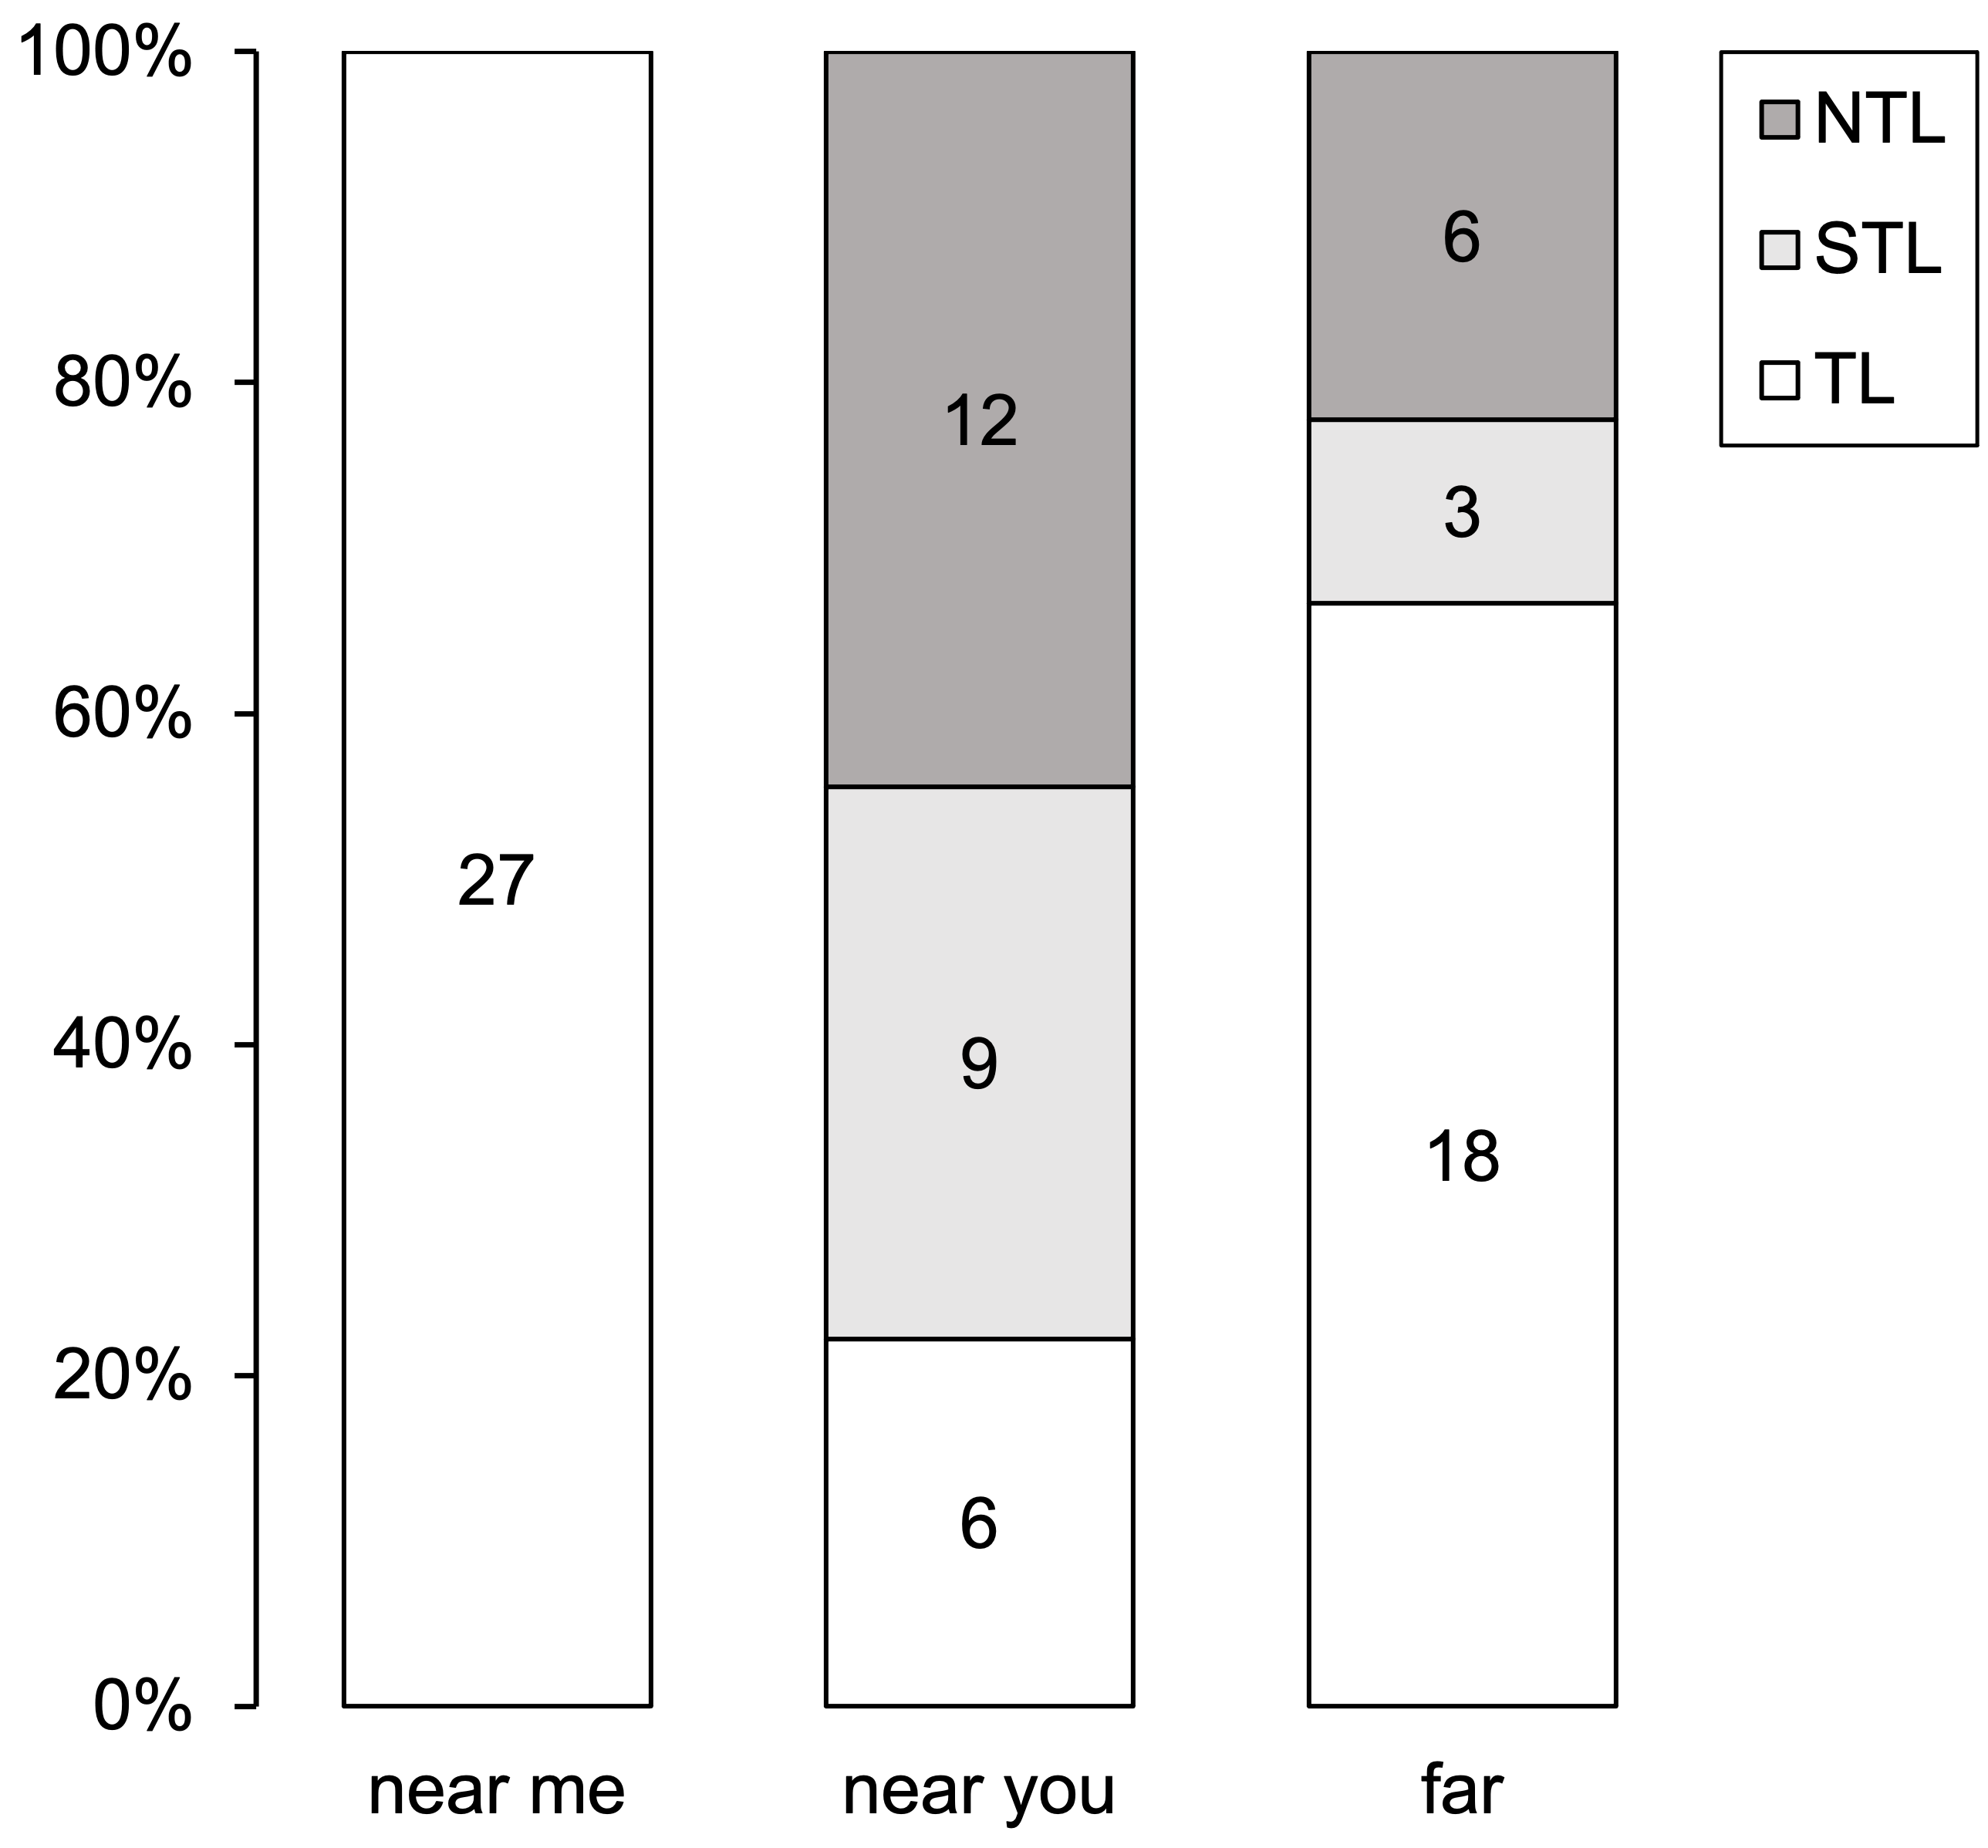
\includegraphics[height=.3\textheight]{figures/overviewAna}\hfill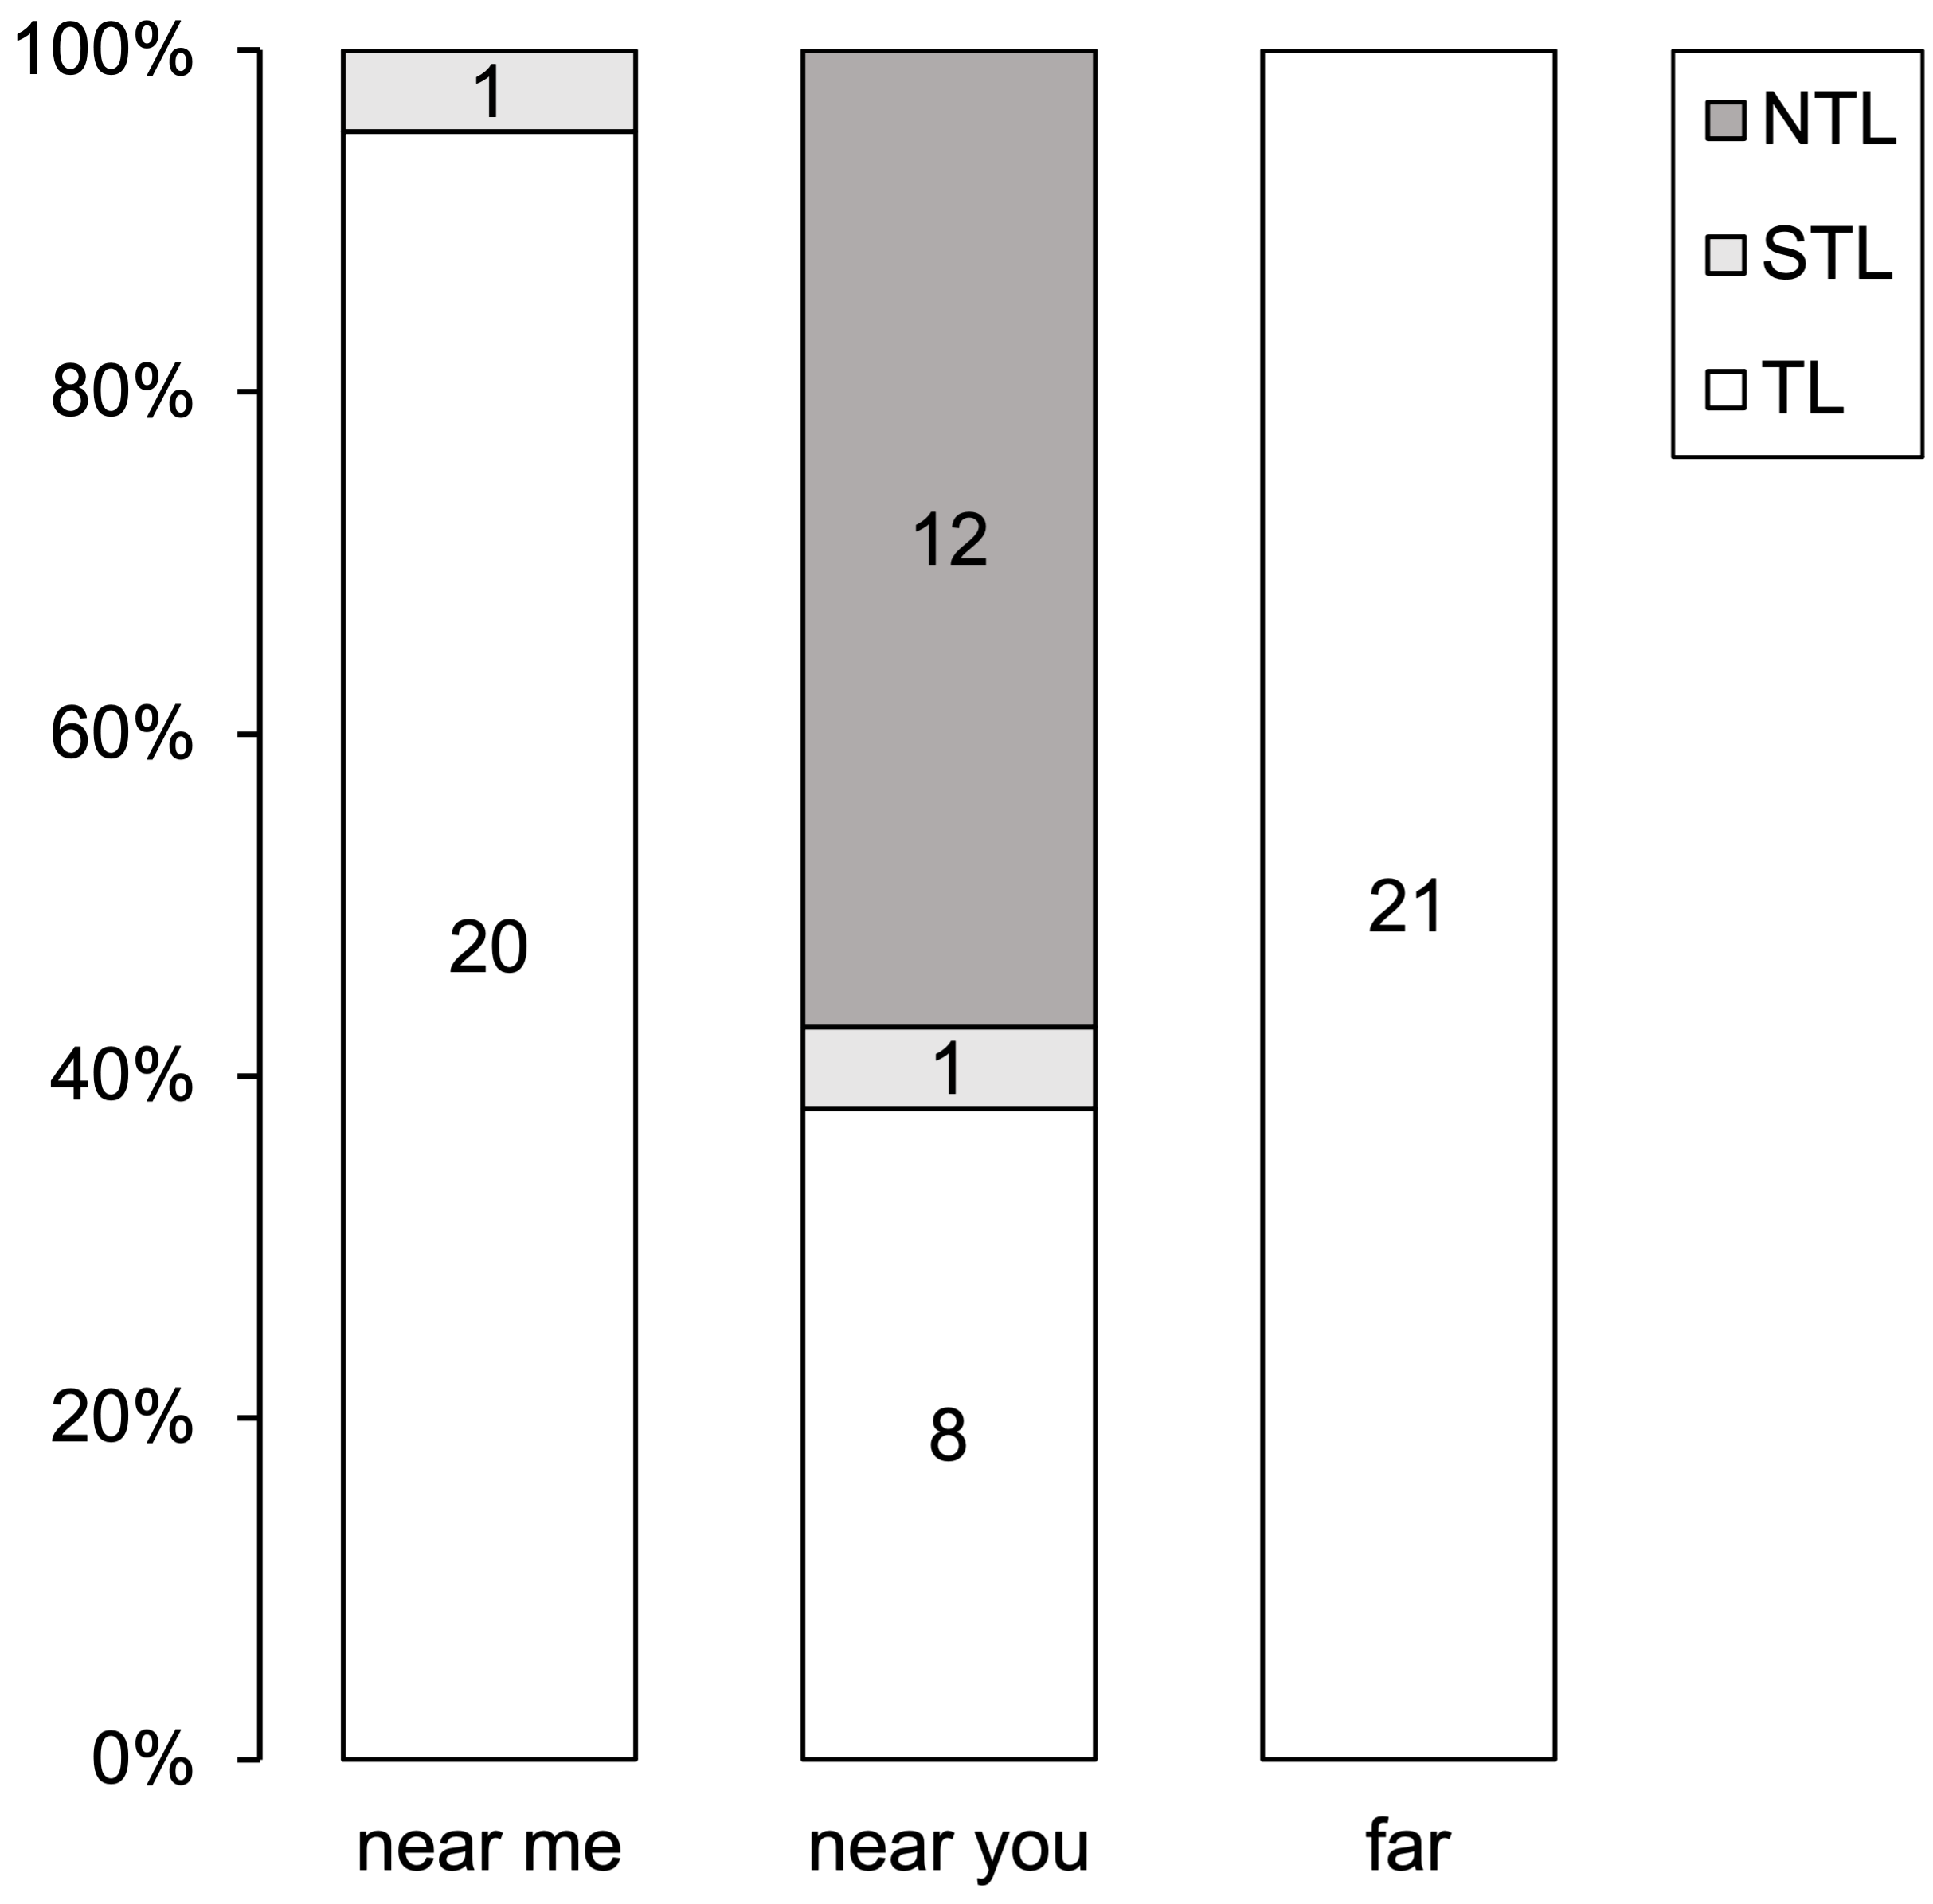
\includegraphics[height=.3\textheight]{figures/overviewBna}
\caption{Ternary demonstrative systems: Comprehension and production results (from \citealt[9]{Terenghi2022Ls})}
\label{fig:dems}
\end{figure}

Crucially, as Figure \ref{fig:dems} shows, the semantic domain that invariably undergoes loss is the hearer-related one, that is: the only one derived by a non-monotonic feature sequence. In fact, Figure \ref{fig:dems} highlights a stark contrast between the latter and demonstrative forms reducible to 1st and 3rd persons (i.e. the monotonically-derived person categories), which are interpreted and produced in a target-like (TL) fashion (that is: compatibly with a three-way deictic opposition) in the overwhelming majority of cases. In hearer-related contexts, instead, both production and comprehension show a considerable amount of non-target-like (NTL) responses, or responses that are not compatible with the hearer-oriented reading. In this context, rather, it can be concluded that the participants perform at chance. This is in line with the predictions made above, once it is assumed that demonstrative systems are syntactically derived by means of person features (\citealt{Harbour2016, BjorkmanEtAl2019, CowperHall2019b, Terenghi2021WCCFL39, Terenghi2023}: Ch. 3). Thus, the featural derivation assumed for (\ref{ex:abr}) is given in (\ref{ex:feat3p}):\footnote{Note the complement set is taken here to be $\pi_{\chi}$: this denotes a collection of regions in space, rather than a collection of individuals as $\pi$ normally does (\citealt{Harbour2016}), following the discussion in \textcites[]{Terenghi2021WCCFL39}[93--94]{Terenghi2023}. Also note that the derivation of the non-participant-related domain is yielded by a $-$participant($-$author(...)) sequence: this partly diverges from the discussion in \citet[92ff.]{Harbour2016} and follows \citet[187]{Terenghi2023}.}

\begin{exe}
\ex \label{ex:feat3p}
\begin{xlist}
\ex \textit{queʃtə} (speaker-related deictic domain): \hfill $+$participant($+$author($\pi_{\chi}$))
\ex \textit{quessə} (hearer-related deictic domain): \hfill $+$participant($-$author($\pi_{\chi}$))
\ex \textit{quellə} (non-participant-related deictic domain): \\ \hbox{} \hfill $-$participant($-$author($\pi_{\chi}$))
\end{xlist}
\end{exe}

\noindent Importantly, the conclusion that the non-monotonically derived category alone undergoes loss in heritage speakers was reached by means of the \textit{Microcontact} methodology (\citealt{DAlessandro2021, AndrianiEtAl2022b}), whereby heritage languages are considered in different immigration settings: in relation to the phenomenon at hand, this translates into a series of majority languages that display different exophoric demonstrative systems. This was done to assess the role of cross-linguistic influence at a finer-grained level. More precisely, the demonstrative systems of heritage Abruzzese (an upper-southern Italo-Romance variety spoken in a central region of Italy) and Sicilian (an extreme Italo-Romance variety spoken in Sicily) varieties were investigated in contact with Spanish in Argentina, French in Quebec and Belgium and English in the US and in Quebec. Among these, only Argentinian Spanish (and in its prescriptive form) instantiates the same ternary system as that found in the baseline varieties; all other varieties cluster together the hearer- and the non-participant-related domains, yielding a basic two-way opposition between the speaker-related deictic domain (\textit{this near me}) and the non-speaker-related deictic domain (\textit{that far from me}). This latter binary system is found in English and (partly) French, but also in Argentinian Spanish (\citealt[135]{Kany1945}; \citealt[888]{LS16}; Andrés Saab, \textit{p.c.}). As shown by \citet{Terenghi2022Ls}, transfer from the different dominant languages is not sufficient to explain these patterns of reduction: the reorganisation of the heritage demonstrative systems does not proceed in a parallel way with respect to that of the relevant dominant language. 


\subsection{Dual in heritage Arabic varieties\label{sec:dual}}

Our second case study focuses on the number domain: we consider the realisation of ternary number systems in heritage Arabic varieties spoken in the US, based on research carried out by \citet{AlbiriniBenmamoun2014} and \citet{Albirini2014}. The dual number category, which denotes sets of entities with a cardinality of 2, is a feature of classical Arabic but is mostly found as a relic (and typically restricted to body parts that come in pairs) in modern Arabic dialects. However, the Palestinian and Egyptian varieties still display a productive dual category, which is realised by the addition of a dedicated morpheme, \textit{-ein}, to the singular form:
\begin{exe}
\ex \textit{saff} $\rightarrow$ \textit{saff-ein} `two classes' (\citealt[247]{AlbiriniBenmamoun2014})
\end{exe}
This contrasts both semantically and morphologically with the plural, which denotes sets of cardinality bigger than 2 and is derived in a non-concatenative fashion (the so-called ``broken'' plurals):
\begin{exe}
\ex \textit{saff} $\rightarrow$ \textit{suffuuf} `classes' (\citealt[255]{AlbiriniBenmamoun2014})
\end{exe}
\citet{AlbiriniBenmamoun2014} investigate whether the dual category is still grammaticalised in Palestinian and Egyptian heritage varieties spoken in the US, or whether, possibly under the effect of contact with English, the dedicated dual marker is no longer employed by heritage speakers of these varieties and pairs of entities are referred to analytically (numeral modifier $+$ plural noun, as in English). On the basis of elicited oral production tasks, \citet{AlbiriniBenmamoun2014} conclude that heritage speakers of Palestinian and Egyptian Arabic in the US are not accurate in forming and using the dual of nouns.

Again, this is in line with our proposal. In fact, in line with the remarks made in Section \ref{sec:backg}, the featural derivation that underlies these different semantics is as follows:
\begin{exe}
\ex \adjustbox{valign=t}{\begin{tabular}{lll}
a. & \textit{saff} (singular) & $+$minimal($+$atomic(P))\\
b. & \textit{saff-ein} (dual) & $+$minimal($-$atomic(P))\\
c. & \textit{suffuuf} (plural) & $-$minimal($-$atomic(P))\\
\end{tabular}}
\end{exe}
That is, the non-monotonically derived number category is the one that undergoes change and loss in the relevant heritage varieties. \citet{AlbiriniBenmamoun2014} and \citet{Albirini2014} suggest that this change might be the effect of transfer from the dominant language, while at the same time highlighting some issues that do not straightforwardly fall out of this. In particular, one of the attested deviant patterns in dual formation is only partly compatible with the English structure: as shown in (\ref{ex:herar1}), the deviant realisation of a target dual morphology is analytic, as in English, but the numeral `two' combines with a singular noun, rather than with the plural one:

\begin{exe}
\ex Heritage Egyptian Arabic (\citealt[741]{Albirini2014})\label{ex:herar1}\\
\gll {\textrevglotstop}indi tnein zamiil fi nafs \v{s}-\v{s}a{\textglotstop\textglotstop}a\\
at-me two roommate in same the-apartment\\
\glt `I have two roommates in the same apartment.'
\end{exe}
This observation cannot conclusively rule out the role of transfer, which can be one of the factors at play in the loss of the dual semantics; future research should examine whether the dual category is unstable, as predicted by the non-monotonicity of the functional sequence that derives it, or not when in contact with comparable ternary number systems. Pending this, it can at least be concluded that heritage Arabic varieties behave in a way that is compatible with our proposal.


\section{Sequences at sentence-level\label{sec:sentence}}

Complexity at the sentential level is more difficult to capture. We will limit ourselves to the case of word order, considering the parametric approach put forward by \citet{Roberts2019}, according to which the relevant sequence of features is the one modelled along a parameter hierarchy. The rationale behind this hypothesis is much in line with the discussion in Section \ref{sec:compl}: concretely, assuming that syntactic properties are derived by a cluster of parameters relative to the activity of a single feature [F] in differently sized domains, if that feature is not active in the derivation of the relevant phenomenon in a given domain (e.g., all heads), it is absent ([$-$F]) from it; conversely, if that feature is instead active in a given domain, it is present ([$+$F]) in it. The domains move from the most general (is the feature active at all?: at the top of the hierarchy) to the most specific one (is the feature active for some specific lexical items only?: at the bottom of the hierarchy). Parametric variation (different parameter settings moving down along the hierarchy) thus derives cross-linguistic variation by means of feature activity along the spine. 

Considering word order, recall that word order is determined by one feature, the [EPP], which ensures that a head attracts an XP to its specifier (see e.g. \citealt{RobertsHolmberg2010}), as well as head movement:\footnote{We use EPP here to refer in general to an “attracting feature”, determining movement of either sort: X or XP movement. EPP is, in this sense, more of a generalized diacritic for movement than a proper feature.} if [EPP] is consistently absent on all heads on the syntactic spine, then the resulting word order will be head-final; if [EPP] is consistently present, then the resulting word order will be head-initial. Non-harmonic word orders are instead derived by an inconsistent setting of the [EPP] parameter: absent in some domains, present in others. This latter configuration is taken to be ``marked'' and its markedness is in turn brought back to a third-factor principle known as ``input generalisation'', whereby the learner is taken to generalise the first setting (whether negative or positive) to all subsequent parameters, unless available evidence suggests otherwise (\citealt{RobertsHolmberg2010}, a.o.).

Here, we examine two cases of word order change in HL: the first one follows the development of heritage Moundridge Schweitzer German (hereafter MSG), examined by \citet{HoppPutnam2015}. The second one regards word order in Even and Sakha, two verb-final languages in contact with Russian. Notice that although Even and Sakha are not spoken only in emigrant communities, they have all the features of HLs: they are spoken by minorities, they are heavily exposed to superstratal Russian, and children acquire them as native speakers in an informal environment (for more information and for the complete data set, the reader is referred to \citealt{GrenobleOsipov2023}).

In their 2015 study, \citeauthor{HoppPutnam2015} show how word order in MSG in contact with English has not moved in the direction of English. MSG is a moribund Palatinate dialect mostly spoken in Kansas, and, like standard German, it presents non-harmonic word order: it is V2 in main clauses and V-final in embedded clauses. Applying \citeauthor{RobertsHolmberg2010}'s (\citeyear{RobertsHolmberg2010}) Generalization of the input principle, we would expect V2 to be lost in MSG. This is however not the case: V2 remains unscathed, similarly to what is reported for Pennsylvania Dutch by \citet{Fuller1997}. Recalling \citeauthor{RobertsHolmberg2010}'s generalisation in (\ref{ex:brgen}), and assuming that the underlying word order of Germanic languages is OV,\footnote{This assumption is not unsubstantiated; German, Dutch and other Germanic languages show head-final characteristics in many environments: numeral, post-positional, as well as adjectival. Furthermore, as shown by many diachronic studies, embedded clauses are more resilient to change and less interested by information structure-related facts. This leads us to conclude that the basic underlying word order in German is head-final.} we can outline German (and MSG in particular) word order as in (\ref{ex:germ}): %\adjustbox{valign=t}{\includegraphics[scale=.75]{B&R.jpg}}
\begin{exe}
\ex \label{ex:gengerm}\begin{xlist}
\ex \label{ex:brgen} For a class of heads H, \textit{u}EPP for H$_{\textrm{F}:-}$ $\neq$ \textit{v} $\rightarrow$ \adjustbox{valign=t}{\begin{tabular}{lll}
\multirow{2}{*}{$\biggl\{$} & \hspace*{-.3cm}{[}$+$EPP]/\textit{v}$_{+\textrm{EPP}}$; & \hspace*{-.3cm}\parbox[t]{2mm}{\multirow{2}{*}{\rotatebox[origin=c]{180}{$\biggl\{$}}}\\
& \hspace*{-.3cm}{[}$-$EPP] elsewhere &\\
\end{tabular}}
\ex In German, \textit{u}EPP for H $\neq$ \textit{v} $\rightarrow$ \adjustbox{valign=t}{\begin{tabular}{lll}
\multirow{2}{*}{$\biggl\{$} & \hspace*{-.3cm}[$-$EPP] / \textit{v}$_{-\textrm{EPP}}$; & \hspace*{-.3cm}\parbox[t]{2mm}{\multirow{2}{*}{\rotatebox[origin=c]{180}{$\biggl\{$}}}\\
& \hspace*{-.3cm}[$+$EPP] / C$_{root}$ &\\
\end{tabular}}\label{ex:germ}
\end{xlist}
\end{exe}
From (\ref{ex:gengerm}) it is evident that this is a condition of markedness, according to the definition above, as one head bears a different [EPP] value than the rest. This results in a form of non-monotonicity, at least in root clauses. We would expect this situation to be ``repaired'' by HL speakers by the loss of V2. This result would be also in conformity with the ease of processing, as V2 requires an additional movement of the verb into a specific sentence-initial phrase, as well as the filling of its specifier, possibly because of discourse requirements. \footnote{We are assuming here the classical analysis of V2 by \citet{denBesten77}, according to which the verb in V2 constructions moves to C, and its specifier is filled by an XP. We can either say that the [EPP] attracts both the verb to the C head and the XP to its specifier, or that there are two different EPP-diacritics on C, one for the head and one for the specifier.} This prediction is not borne out: \citet{HoppPutnam2015} convincingly show not only that V2 is not lost and that MSG has not become SVO like in English, but also that V2 is extended to the embedded environment, as shown by (\ref{ex:v2sub}), where the finite verb \textit{würde} raises across the negation \textit{nicht} to unambiguously reach the second position:

\begin{exe}
\ex MSG Participant 122, from \citealt[204]{HoppPutnam2015}\\
\gll ... dass die Verkäuferin \emph{würde} das nicht merken\\
{} that the saleslady would that not notice\\
\glt `that the saleslady would not notice that'\label{ex:v2sub}
\end{exe}
This last piece of information makes the picture more interesting, and begs for some reflection. To start with, while MSG has indeed not turned into an SVO-language, some change has happened nevertheless in the direction of uniformation: the embedded clauses have developed V2. This means that the lack of uniformity in the sequence has indeed been resolved, at least within the verbal domain: C has retained [EPP] in main clauses, but this has been furthermore transmitted to the T/C of the embedded clause, creating a monotonic sequence in the verbal domain.

The second observation is that this change has not started from within, that is, it has not started from an extension of the value of EPP on \textit{v}; rather, it has been induced by some mirroring of the feature value on the C of the matrix clause. This is also not totally unexpected, as change in heritage languages has been argued to penetrate the structure from a peripheral/edge position and slowly extend to the whole sentential domain. Interestingly, this is not the direction followed by first language acquisition, as argued by \citet{RobertsHolmberg2010}: this suggests that HLs have their own mechanisms of adaptation; this reflects the fact that change in contact is less uniform and more idiosyncratic than diachronic change, which has already been noted when discourse elements are involved (see \citet{DAlessandroEtAlIP}). Furthermore, this tendency to uniformity and reduction of complexity has taken place within one domain: this is also not unexpected, given that language change in HL takes place step-wise, and optionality and coexistence of different, even conflicting, features is quite common (\citealt{Polinsky2018, AalberseMuysken2019}).

Let us now turn to the case of Even and Sakha investigated by \citet{GrenobleOsipov2023}; this is somewhat more complex, given that these minority languages are in contact with Russian, a non-configurational language with a word order which is much less fixed than that of English, for instance. A contact language with a discourse-driven word order is more difficult to generalise upon. For basic declarative clauses, Russian can be considered to be SVO; both Even and Sakha are SOV (\citealt{Malchukov1995}; \citealt{Stachowski1998}). This means that, while Russian is head-initial, i.e. according to Roberts has a [$-$EPP] on \textit{v}, Even and Sakha have [$+$EPP], being head-final. In a study on word order, \citeauthor{GrenobleOsipov2023} report a shift in younger speakers towards SVO word order. No evidence has been mentioned by the authors about word order change in the language otherwise, but case morphology has been argued to be undergoing loss. This amounts to saying that the change that Sakha and Even are undergoing is a head-initial to head-final shift in the whole language domain. As an example, consider (\ref{even}), from \citet[33]{GrenobleOsipov2023}:
 
\begin{exe} 
\tabcolsep=.8\tabcolsep
\ex \label{even}
\begin{tabular}[t]{@{}l@{~}lllll@{}}
a. & S-O1-O2-V & Asatkan & {\texteng}in-u & ulre-č & \emph{ulič-d-de-n}\\
 & & girl-\textsc{nom} & dog-\textsc{acc} & meat-\textsc{inst} & feed-\textsc{ipfv-prs-3sg}\\
b. & S-O2-O1-V & Asatkan & ulre-č & {\texteng}in-u & \emph{ulič-d-de-n}\\
c. & S-O1-V-O2 & Asatkan & {\texteng}in-u & \emph{ulič-d-de-n} & ulre-č \\
d. & S-V-O1-O2 & Asatkan & \emph{ulič-d-de-n} & {\texteng}in-u & ulre-č\\[.5em]
   & \multicolumn{5}{@{}l@{}}{`The girl feeds the dog meat.'}\\
\end{tabular}
\end{exe}
\citet{GrenobleOsipov2023} argue that in traditional Even the only possible word order is V-final. The examples in (\ref{even}) are instead all acceptable and produced by younger generations of Even speakers. While all word orders co-exist, the mere fact that all four word orders are found in modern Even highlights a change in progress, which they attribute to the contact with Russian. We leave this here as a speculation, given that sufficient data are lacking, to support this generalisation. What matters is that change, in this context, seems to start off indeed from \textit{v}, like in L1 acquisition contexts and as predicted by \citet{RobertsHolmberg2010}.

Before concluding, it should be noted that our proposal seems to make predictions on the areas of heritage syntax that are more or less vulnerable to transfer. In the case of word order, transfer has been widely indicated as the possible source of change in heritage languages (going beyond the cases discussed here, see discussion in \citealt[section 6.7]{Polinsky2018} and references therein). However, it is crucially \textit{not} the case that transfer affects word order across the board. 

Heritage Egyptian Arabic varieties illustrate this point quite convincingly. \citet{AlbiriniEtAl2011} show that Egyptian Arabic heritage speakers tend to shift from VSO- to SVO-order in the clausal domain; this is likely to be attributed to transfer from the dominant language, English, that lacks the VSO-order altogether. However, in the nominal domain, Egyptian Arabic heritage speakers consistently retain the ``baseline'' word order noun--adjective, which is not prone to change under the pressure of English adjective--noun word order (\citealt{Albirini2014}). Note that the impact of English in this domain is acknowledged in the progressive loss of agreement between the adjective and the noun head. However, transfer does not apply to word order in this case. This fact can be traced back to the general harmony of functional heads already discussed: while a change VSO $>$ SVO does not have an impact on the system, as head-directionality is preserved, a change NA $>$ AN would amount to a breach of the harmonic setting of parameters across the nominal and the clausal domains. This is expected to be disfavoured, following our proposal. Hence, the heritage Egyptian Arabic data seem to confirm that monotonic sequences of features are favoured in heritage grammars and further constrain the domain of application of transfer: transfer can apply, but only if it does not lead to a cognitively disfavoured sequence of features.

\section{Conclusions\label{sec:concl}} 

The foregoing argued that unrelated changes attested in heritage languages ultimately all hinge on the concept of non-monotonicity along feature sequences: when a feature sequence contains different values, the switching point can be identified as the gateway to change in heritage varieties. Change has been shown to be sometimes further driven by transfer, but transfer itself seems to be to some extent constrained to targeting those switching points along the relevant feature sequences. As such, the ultimate trigger for syntactic change in the domains considered in this study seems to be simply complexity, which is captured straightforwardly by the bias towards monotonic derivations. 

\begin{sloppypar}
One additional observation is that, for the cases illustrated in this work, the predicted change for heritage languages is identical to that which has been documented in diachrony; conversely, no such strict parallel between syntactic change in contact and in diachrony seems to be observable for phenomena which eschew a structural analysis in terms of featural sequences as the ones discussed here. Crucially, the latter phenomena are those about whose development no clear-cut predictions can be made (see %also D'Alessandro, Putnam \& Terenghi in prep
\citet{DAlessandroEtAlIP}). This seems to suggest that change in contact under a restricted language use situation (heritage languages) and change in diachrony target one and the same structural sequence of syntactic heads (possibly at different speeds, \citealt{KupischPolinsky2022}), and that otherwise their outputs diverge for more complex, not exclusively syntactic phenomena. While the sensitivity of bilinguals to phenomena sitting at (external) interfaces is well-known (Interface Hypothesis, \citealt{SoraceSerratrice2009, Sorace2011} for an overview), the relation between this and diachronic change had not been explored before.
\end{sloppypar}

In summary, we have shown that languages do indeed undergo a reduction in complexity, but only as far as purely grammatical elements are concerned. Since the same conclusions do not seem to be warranted for syntactic phenomena involving discourse, for which change takes mostly unpredictable paths as determined by several external factors (such as the attitude of the speakers, the context, the level of mastery of the language, \textit{etc.}) as well as by grammar-internal factors (such as structural similarity), this strongly suggests that a division needs to be drawn between different syntactic phenomena. Therefore, we hope to have shown that it is not methodologically valid to consider complexity of a grammatical system as a whole. Rather, as different subparts of grammatical systems behave differently, depending on whether external factors or other modules are involved or not, it is necessary to suitably delimit the domain of investigation for the issue of complexity in language to be purposefully addressed.

\sloppy\printbibliography[heading=subbibliography,notkeyword=this]
\end{document}
